\documentclass[]{elsarticle} %review=doublespace preprint=single 5p=2 column
%%% Begin My package additions %%%%%%%%%%%%%%%%%%%

\usepackage[hyphens]{url}


\usepackage{lineno} % add
  \linenumbers % turns line numbering on

\usepackage{graphicx}
%%%%%%%%%%%%%%%% end my additions to header

\usepackage[T1]{fontenc}
\usepackage{lmodern}
\usepackage{amssymb,amsmath}
\usepackage{ifxetex,ifluatex}
\usepackage{fixltx2e} % provides \textsubscript
% use upquote if available, for straight quotes in verbatim environments
\IfFileExists{upquote.sty}{\usepackage{upquote}}{}
\ifnum 0\ifxetex 1\fi\ifluatex 1\fi=0 % if pdftex
  \usepackage[utf8]{inputenc}
\else % if luatex or xelatex
  \usepackage{fontspec}
  \ifxetex
    \usepackage{xltxtra,xunicode}
  \fi
  \defaultfontfeatures{Mapping=tex-text,Scale=MatchLowercase}
  \newcommand{\euro}{€}
\fi
% use microtype if available
\IfFileExists{microtype.sty}{\usepackage{microtype}}{}
\usepackage[]{natbib}
\bibliographystyle{plainnat}

\usepackage{graphicx}
\ifxetex
  \usepackage[setpagesize=false, % page size defined by xetex
              unicode=false, % unicode breaks when used with xetex
              xetex]{hyperref}
\else
  \usepackage[unicode=true]{hyperref}
\fi
\hypersetup{breaklinks=true,
            bookmarks=true,
            pdfauthor={},
            pdftitle={Testing Forest Area as a random effect},
            colorlinks=false,
            urlcolor=blue,
            linkcolor=magenta,
            pdfborder={0 0 0}}

\setcounter{secnumdepth}{5}
% Pandoc toggle for numbering sections (defaults to be off)

% Pandoc syntax highlighting
\usepackage{color}
\usepackage{fancyvrb}
\newcommand{\VerbBar}{|}
\newcommand{\VERB}{\Verb[commandchars=\\\{\}]}
\DefineVerbatimEnvironment{Highlighting}{Verbatim}{commandchars=\\\{\}}
% Add ',fontsize=\small' for more characters per line
\usepackage{framed}
\definecolor{shadecolor}{RGB}{248,248,248}
\newenvironment{Shaded}{\begin{snugshade}}{\end{snugshade}}
\newcommand{\AlertTok}[1]{\textcolor[rgb]{0.94,0.16,0.16}{#1}}
\newcommand{\AnnotationTok}[1]{\textcolor[rgb]{0.56,0.35,0.01}{\textbf{\textit{#1}}}}
\newcommand{\AttributeTok}[1]{\textcolor[rgb]{0.77,0.63,0.00}{#1}}
\newcommand{\BaseNTok}[1]{\textcolor[rgb]{0.00,0.00,0.81}{#1}}
\newcommand{\BuiltInTok}[1]{#1}
\newcommand{\CharTok}[1]{\textcolor[rgb]{0.31,0.60,0.02}{#1}}
\newcommand{\CommentTok}[1]{\textcolor[rgb]{0.56,0.35,0.01}{\textit{#1}}}
\newcommand{\CommentVarTok}[1]{\textcolor[rgb]{0.56,0.35,0.01}{\textbf{\textit{#1}}}}
\newcommand{\ConstantTok}[1]{\textcolor[rgb]{0.00,0.00,0.00}{#1}}
\newcommand{\ControlFlowTok}[1]{\textcolor[rgb]{0.13,0.29,0.53}{\textbf{#1}}}
\newcommand{\DataTypeTok}[1]{\textcolor[rgb]{0.13,0.29,0.53}{#1}}
\newcommand{\DecValTok}[1]{\textcolor[rgb]{0.00,0.00,0.81}{#1}}
\newcommand{\DocumentationTok}[1]{\textcolor[rgb]{0.56,0.35,0.01}{\textbf{\textit{#1}}}}
\newcommand{\ErrorTok}[1]{\textcolor[rgb]{0.64,0.00,0.00}{\textbf{#1}}}
\newcommand{\ExtensionTok}[1]{#1}
\newcommand{\FloatTok}[1]{\textcolor[rgb]{0.00,0.00,0.81}{#1}}
\newcommand{\FunctionTok}[1]{\textcolor[rgb]{0.00,0.00,0.00}{#1}}
\newcommand{\ImportTok}[1]{#1}
\newcommand{\InformationTok}[1]{\textcolor[rgb]{0.56,0.35,0.01}{\textbf{\textit{#1}}}}
\newcommand{\KeywordTok}[1]{\textcolor[rgb]{0.13,0.29,0.53}{\textbf{#1}}}
\newcommand{\NormalTok}[1]{#1}
\newcommand{\OperatorTok}[1]{\textcolor[rgb]{0.81,0.36,0.00}{\textbf{#1}}}
\newcommand{\OtherTok}[1]{\textcolor[rgb]{0.56,0.35,0.01}{#1}}
\newcommand{\PreprocessorTok}[1]{\textcolor[rgb]{0.56,0.35,0.01}{\textit{#1}}}
\newcommand{\RegionMarkerTok}[1]{#1}
\newcommand{\SpecialCharTok}[1]{\textcolor[rgb]{0.00,0.00,0.00}{#1}}
\newcommand{\SpecialStringTok}[1]{\textcolor[rgb]{0.31,0.60,0.02}{#1}}
\newcommand{\StringTok}[1]{\textcolor[rgb]{0.31,0.60,0.02}{#1}}
\newcommand{\VariableTok}[1]{\textcolor[rgb]{0.00,0.00,0.00}{#1}}
\newcommand{\VerbatimStringTok}[1]{\textcolor[rgb]{0.31,0.60,0.02}{#1}}
\newcommand{\WarningTok}[1]{\textcolor[rgb]{0.56,0.35,0.01}{\textbf{\textit{#1}}}}

% tightlist command for lists without linebreak
\providecommand{\tightlist}{%
  \setlength{\itemsep}{0pt}\setlength{\parskip}{0pt}}

% From pandoc table feature
\usepackage{longtable,booktabs,array}
\usepackage{calc} % for calculating minipage widths
% Correct order of tables after \paragraph or \subparagraph
\usepackage{etoolbox}
\makeatletter
\patchcmd\longtable{\par}{\if@noskipsec\mbox{}\fi\par}{}{}
\makeatother
% Allow footnotes in longtable head/foot
\IfFileExists{footnotehyper.sty}{\usepackage{footnotehyper}}{\usepackage{footnote}}
\makesavenoteenv{longtable}


\usepackage{setspace}
\usepackage{color}
\newcommand{\beginsupplement}{  \setcounter{table}{0} \renewcommand{\thetable}{S\arabic{table}} \setcounter{figure}{0} \renewcommand{\thefigure}{S\arabic{figure}}\setcounter{equation}{0} \renewcommand{\theequation}{S\arabic{equation}}}



\begin{document}


\begin{frontmatter}

  \title{Testing Forest Area as a random effect}
    \author[]{R. Willem Vervoort%
  %
  \fnref{1}}
   \ead{willem.vervoort@sydney.edu.au} 
    \author[]{Eliana Nervi}
   \ead{eliananervif@gmail.com} 
    \author[]{Jimena Alonso}
   \ead{jalonso@fing.edu.uy} 
      \cortext[cor1]{Corresponding author}
    \fntext[1]{Corresponding Author}
  
  \begin{abstract}
  This supplementary material file compares different linear and non-linear relationships for the impact of forest cover on the change in stream flow.
  \end{abstract}
  
 \end{frontmatter}

\setcounter{table}{0} \renewcommand{\thetable}{S\arabic{table}} \setcounter{figure}{0} \renewcommand{\thefigure}{S\arabic{figure}}\setcounter{equation}{0} \renewcommand{\theequation}{S\arabic{equation}}

\hypertarget{introduction}{%
\section{Introduction}\label{introduction}}

This supplementary material is related to `Generalising the impact of forest cover on streamflow from experimental data: it is not that simple. Vervoort et al.'

This document outlines a test suggested in the first review of the manuscript. The AE of the Journal of Hydrology suggested that we test if including the total forest area as a variable would make sense. Not only the \% change in area is important, but what total area of forest was there in the first place.

This test focusses on the large catchment data (\textless{} 1000 km\textsuperscript{2}) for two reasons:

\begin{enumerate}
\def\labelenumi{\arabic{enumi}.}
\tightlist
\item
  This was a manageable subset and many of the papers are fairly accessible, in contrast to the small catchments.
\item
  Many of the small catchments have 100\% area covered in forest, so are not useful to identify if total area of forest has an impact on the change in flow.
\end{enumerate}

\hypertarget{set-up-the-packages}{%
\subsection{set up the packages}\label{set-up-the-packages}}

\hypertarget{read-in-the-data}{%
\subsection{read in the data}\label{read-in-the-data}}

Read in the data and massage column names to make columns useable in the model.

\begin{Shaded}
\begin{Highlighting}[]
\NormalTok{Data\_wF }\OtherTok{\textless{}{-}} \FunctionTok{read\_csv}\NormalTok{(}\StringTok{"../../data/LCdatawithFA.xlsx {-} LW\_TotForest\_Area.csv"}\NormalTok{)}
\end{Highlighting}
\end{Shaded}

\begin{verbatim}
## Rows: 61 Columns: 25
## -- Column specification --------------------------------------------------------
## Delimiter: ","
## chr (10): Watershed name, Forest type, Hydrological regime, yearFarea, Comme...
## dbl (15): Watershed #, Area(km2), Pa(mm), Farea_km2, Perc_Farea_pre, DeltaF_...
## 
## i Use `spec()` to retrieve the full column specification for this data.
## i Specify the column types or set `show_col_types = FALSE` to quiet this message.
\end{verbatim}

\begin{Shaded}
\begin{Highlighting}[]
\CommentTok{\# change some column names}
\FunctionTok{names}\NormalTok{(Data\_wF)[}\DecValTok{3}\SpecialCharTok{:}\DecValTok{4}\NormalTok{] }\OtherTok{\textless{}{-}} \FunctionTok{c}\NormalTok{(}\StringTok{"Area\_km2"}\NormalTok{, }\StringTok{"Pa\_mm"}\NormalTok{)}
\FunctionTok{names}\NormalTok{(Data\_wF)[}\DecValTok{5}\SpecialCharTok{:}\DecValTok{6}\NormalTok{] }\OtherTok{\textless{}{-}} \FunctionTok{c}\NormalTok{(}\StringTok{"Forest\_type"}\NormalTok{, }\StringTok{"Hydrological\_regime"}\NormalTok{)}
\FunctionTok{names}\NormalTok{(Data\_wF)[}\DecValTok{13}\SpecialCharTok{:}\DecValTok{14}\NormalTok{] }\OtherTok{\textless{}{-}} \FunctionTok{c}\NormalTok{(}\StringTok{"Precip\_data\_type"}\NormalTok{, }\StringTok{"Assessment\_technique"}\NormalTok{)}
\end{Highlighting}
\end{Shaded}

\hypertarget{some-changes-to-the-overall-data}{%
\subsection{Some changes to the overall data}\label{some-changes-to-the-overall-data}}

\begin{enumerate}
\def\labelenumi{\arabic{enumi}.}
\tightlist
\item
  calculating the dryness
\end{enumerate}

\begin{Shaded}
\begin{Highlighting}[]
\CommentTok{\# calculate dryness index}
\NormalTok{Data\_wF }\OtherTok{\textless{}{-}}\NormalTok{ Data\_wF }\SpecialCharTok{\%\textgreater{}\%}
  \FunctionTok{mutate}\NormalTok{(}\AttributeTok{Dryness =}\NormalTok{ E0}\SpecialCharTok{/}\NormalTok{Pa\_mm)}
\end{Highlighting}
\end{Shaded}

\begin{enumerate}
\def\labelenumi{\arabic{enumi}.}
\setcounter{enumi}{1}
\tightlist
\item
  remove watershed 1 (the Amazon) from the analysis
\end{enumerate}

\begin{Shaded}
\begin{Highlighting}[]
\NormalTok{Data\_wF }\OtherTok{\textless{}{-}}\NormalTok{ Data\_wF }\SpecialCharTok{\%\textgreater{}\%}
  \FunctionTok{filter}\NormalTok{(}\StringTok{\textasciigrave{}}\AttributeTok{Watershed \#}\StringTok{\textasciigrave{}} \SpecialCharTok{!=} \DecValTok{1}\NormalTok{)}
\end{Highlighting}
\end{Shaded}

\begin{enumerate}
\def\labelenumi{\arabic{enumi}.}
\setcounter{enumi}{2}
\tightlist
\item
  include length as a variable
\end{enumerate}

\begin{Shaded}
\begin{Highlighting}[]
\NormalTok{All\_data }\OtherTok{\textless{}{-}}\NormalTok{ Data\_wF }\SpecialCharTok{\%\textgreater{}\%}
  \FunctionTok{mutate}\NormalTok{(}\AttributeTok{length =}\NormalTok{ To }\SpecialCharTok{{-}}\NormalTok{ From,}
         \AttributeTok{mid\_year =}\NormalTok{ From }\SpecialCharTok{+}\NormalTok{ (To }\SpecialCharTok{{-}}\NormalTok{ From)}\SpecialCharTok{/}\DecValTok{2}\NormalTok{)}
\end{Highlighting}
\end{Shaded}

\hypertarget{results}{%
\section{Results}\label{results}}

Run the model simply as a GLM, transform Area using log10, as in the manuscript.

\begin{Shaded}
\begin{Highlighting}[]
\NormalTok{Forest\_model\_all }\OtherTok{\textless{}{-}} \FunctionTok{gam}\NormalTok{(DeltaQf\_perc }\SpecialCharTok{\textasciitilde{}}\NormalTok{ DeltaF\_perc }\SpecialCharTok{+} 
                    \FunctionTok{log10}\NormalTok{(Area\_km2) }\SpecialCharTok{+} 
\NormalTok{                    Dryness }\SpecialCharTok{+} 
\NormalTok{                    Perc\_Farea\_pre }\SpecialCharTok{+}
\NormalTok{                    Precip\_data\_type }\SpecialCharTok{+}\NormalTok{  Assessment\_technique }\SpecialCharTok{+}
\NormalTok{                    Forest\_type }\SpecialCharTok{+}
\NormalTok{                    Hydrological\_regime}
\NormalTok{                    , }\AttributeTok{data =}\NormalTok{ All\_data)}
\FunctionTok{summary}\NormalTok{(Forest\_model\_all)}
\end{Highlighting}
\end{Shaded}

\begin{verbatim}
## 
## Family: gaussian 
## Link function: identity 
## 
## Formula:
## DeltaQf_perc ~ DeltaF_perc + log10(Area_km2) + Dryness + Perc_Farea_pre + 
##     Precip_data_type + Assessment_technique + Forest_type + Hydrological_regime
## 
## Parametric coefficients:
##                             Estimate Std. Error t value Pr(>|t|)   
## (Intercept)                -16.04690   15.08196  -1.064  0.29676   
## DeltaF_perc                 -0.37440    0.11561  -3.239  0.00318 **
## log10(Area_km2)              1.55899    2.31470   0.674  0.50634   
## Dryness                      4.40194    3.21852   1.368  0.18269   
## Perc_Farea_pre               0.03722    0.07544   0.493  0.62572   
## Precip_data_typeOB         -19.28048    6.55235  -2.943  0.00661 **
## Precip_data_typeSG         -12.00304    6.75886  -1.776  0.08702 . 
## Assessment_techniqueEA, HM   1.36550    9.86348   0.138  0.89092   
## Assessment_techniqueHM      15.44379    6.16998   2.503  0.01866 * 
## Assessment_techniqueQPW      2.79556    9.90330   0.282  0.77988   
## Assessment_techniqueSH      18.51105    7.64697   2.421  0.02249 * 
## Forest_typeCF               -9.46812    6.16583  -1.536  0.13628   
## Forest_typeMF                0.27749    4.64399   0.060  0.95279   
## Hydrological_regimeSD       20.97769    6.66044   3.150  0.00397 **
## ---
## Signif. codes:  0 '***' 0.001 '**' 0.01 '*' 0.05 '.' 0.1 ' ' 1
## 
## 
## R-sq.(adj) =  0.735   Deviance explained = 82.1%
## GCV = 128.37  Scale est. = 84.534    n = 41
\end{verbatim}

This suggest that forest area is not at all significant in the model. In fact, the hydrological modelling technique is much more important. Overall the model explains roughly 82\% of the variation.

\begin{Shaded}
\begin{Highlighting}[]
\FunctionTok{gam.check}\NormalTok{(Forest\_model\_all)}
\end{Highlighting}
\end{Shaded}

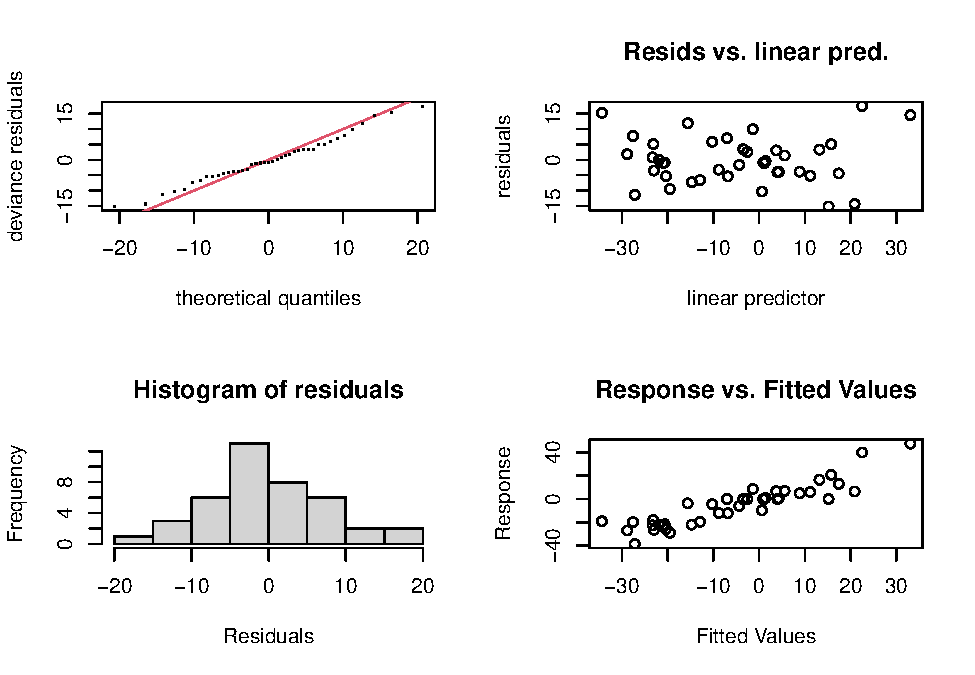
\includegraphics{Test_model_totalForestArea_files/figure-latex/check-model-percent-1.pdf}

\begin{verbatim}
## 
## Method: GCV   Optimizer: magic
## Model required no smoothing parameter selectionModel rank =  14 / 14
\end{verbatim}

\begin{Shaded}
\begin{Highlighting}[]
\CommentTok{\#plot(Forest\_model\_all)}
\end{Highlighting}
\end{Shaded}

The fit of the model is also well-behaved, as would be expected. The data are mostly from hydrological modelling, stabilising the response of the change in forest to change in streamflow.

\hypertarget{run-the-model-on-forest-area-rather-than}\label{run-the-model-on-forest-area-rather-than}}

Possibly, using the total \% forest is not taking into account the differences in total area of forest. So we can also test with total ha. Note that this can interact with total area: larger catchments will have larger total areas of forest.

We appear to have less data here as \% is reported more, but we can calculate total ha by multiplying \% by total area.

\begin{Shaded}
\begin{Highlighting}[]
\NormalTok{All\_data }\OtherTok{\textless{}{-}}\NormalTok{ Data\_wF }\SpecialCharTok{\%\textgreater{}\%}
  \FunctionTok{mutate}\NormalTok{(}\AttributeTok{Farea\_km2 =} \FunctionTok{ifelse}\NormalTok{(}\FunctionTok{is.na}\NormalTok{(Farea\_km2)}\SpecialCharTok{==}\NormalTok{T,Area\_km2}\SpecialCharTok{*}\NormalTok{Perc\_Farea\_pre}\SpecialCharTok{/}\DecValTok{100}\NormalTok{,Farea\_km2))}

\NormalTok{Forest\_model\_area }\OtherTok{\textless{}{-}} \FunctionTok{gam}\NormalTok{(DeltaQf\_perc }\SpecialCharTok{\textasciitilde{}}\NormalTok{ DeltaF\_perc }\SpecialCharTok{+} 
                    \FunctionTok{log10}\NormalTok{(Area\_km2) }\SpecialCharTok{+} 
\NormalTok{                    Dryness }\SpecialCharTok{+} 
\NormalTok{                    Farea\_km2 }\SpecialCharTok{+}
\NormalTok{                    Precip\_data\_type }\SpecialCharTok{+}\NormalTok{  Assessment\_technique }\SpecialCharTok{+}
\NormalTok{                    Forest\_type }\SpecialCharTok{+}
\NormalTok{                    Hydrological\_regime}
\NormalTok{                    , }\AttributeTok{data =}\NormalTok{ All\_data)}
\FunctionTok{summary}\NormalTok{(Forest\_model\_area)}
\end{Highlighting}
\end{Shaded}

\begin{verbatim}
## 
## Family: gaussian 
## Link function: identity 
## 
## Formula:
## DeltaQf_perc ~ DeltaF_perc + log10(Area_km2) + Dryness + Farea_km2 + 
##     Precip_data_type + Assessment_technique + Forest_type + Hydrological_regime
## 
## Parametric coefficients:
##                              Estimate Std. Error t value Pr(>|t|)    
## (Intercept)                -3.021e+01  1.641e+01  -1.841 0.076621 .  
## DeltaF_perc                -3.718e-01  9.294e-02  -4.000 0.000442 ***
## log10(Area_km2)             6.084e+00  3.346e+00   1.818 0.080140 .  
## Dryness                     3.255e+00  3.156e+00   1.031 0.311481    
## Farea_km2                  -6.197e-05  3.922e-05  -1.580 0.125688    
## Precip_data_typeOB         -1.740e+01  6.224e+00  -2.795 0.009431 ** 
## Precip_data_typeSG         -8.667e+00  6.680e+00  -1.297 0.205467    
## Assessment_techniqueEA, HM  4.465e-01  9.411e+00   0.047 0.962513    
## Assessment_techniqueHM      1.436e+01  5.973e+00   2.404 0.023345 *  
## Assessment_techniqueQPW    -6.118e-01  9.487e+00  -0.064 0.949055    
## Assessment_techniqueSH      1.741e+01  7.243e+00   2.404 0.023362 *  
## Forest_typeCF              -8.111e+00  5.993e+00  -1.353 0.187195    
## Forest_typeMF              -4.063e-01  4.433e+00  -0.092 0.927641    
## Hydrological_regimeSD       2.346e+01  6.605e+00   3.552 0.001428 ** 
## ---
## Signif. codes:  0 '***' 0.001 '**' 0.01 '*' 0.05 '.' 0.1 ' ' 1
## 
## 
## R-sq.(adj) =  0.756   Deviance explained = 83.5%
## GCV = 118.56  Scale est. = 78.075    n = 41
\end{verbatim}

\begin{Shaded}
\begin{Highlighting}[]
\FunctionTok{gam.check}\NormalTok{(Forest\_model\_area)}
\end{Highlighting}
\end{Shaded}

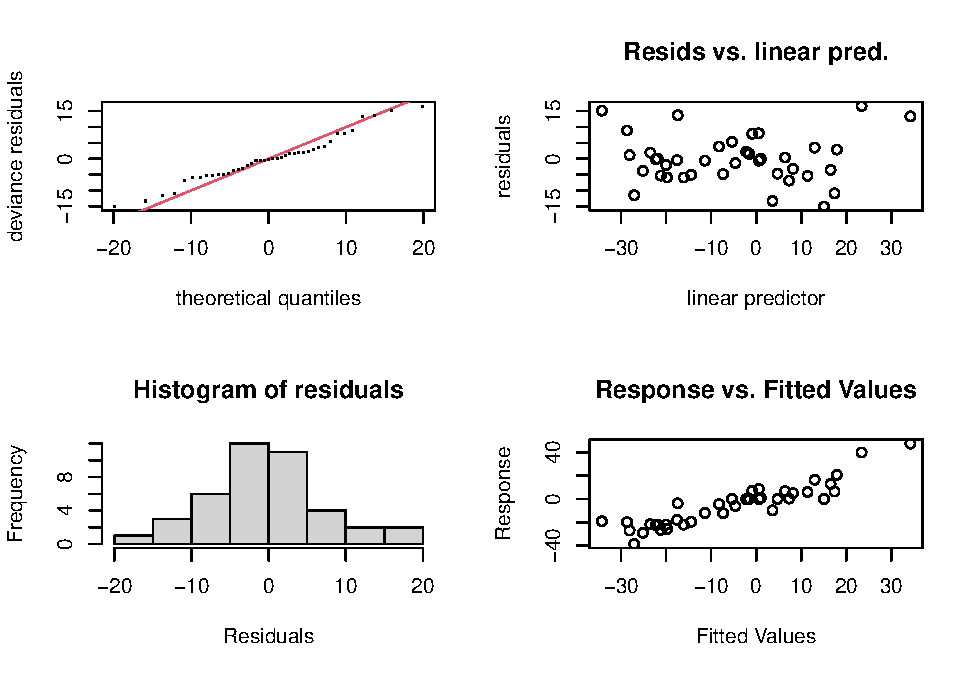
\includegraphics{Test_model_totalForestArea_files/figure-latex/check_resid_area-1.pdf}

\begin{verbatim}
## 
## Method: GCV   Optimizer: magic
## Model required no smoothing parameter selectionModel rank =  14 / 14
\end{verbatim}

\begin{Shaded}
\begin{Highlighting}[]
\CommentTok{\#plot(Forest\_model\_all)}
\end{Highlighting}
\end{Shaded}

Again, not significant and the model is well-behaved. Note that the Hydrological modelling assessment technique (HM) is again highly significant.

\hypertarget{conclusion}{%
\section{Conclusion}\label{conclusion}}

There is no effect of forest area in the relationship between change in flow and percent change in forest cover.

\bibliography{forestandwater.bib}


\end{document}
